\chapter{Software Design}

\section{Introduction to Software Design}

This chapter presents the detailed software design of the proposed system. It translates the requirements identified in Chapter 3 into structured architectural, behavioral, and data models. The purpose of this chapter is to provide a clear blueprint for system implementation, ensuring maintainability, scalability, and modular development.

This chapter includes architectural design, UML models, data flow models, and database design applicable to machine learning systems, web/mobile applications, and other software engineering domains.

%%%%%%%%%%%%%%%%%%%%%%%%%%%%%%%%%%%%%%%%%%%%%%%%%%%%%%
\section{Design Methodology and Software Process Model}

\subsection{Design Methodology}

This project follows a structured design methodology. Depending on the project type, one of the following approaches may be adopted:

\begin{itemize}
    \item Object-Oriented Design (OOD)
    \item Model-View-Controller (MVC)
    \item Layered Architecture
    \item Microservices Architecture
    \item Client-Server Architecture
    \item Data-Centric Design (for ML systems)
\end{itemize}

The selected methodology ensures modularity, loose coupling, reusability, and scalability.

\textbf{Guidelines:}
\begin{itemize}
    \item Clearly justify the selected design approach.
    \item Explain why it suits your domain (ML, Web, Mobile, etc.).
    \item Mention design principles followed (SOLID, DRY, Separation of Concerns).
\end{itemize}

%%%%%%%%%%%%%%%%%%%%%%%%%%%%%%%%%%%%%%%%%%%%%%%%%%%%%%
\subsection{Software Process Model}

The project follows the \textbf{(Agile / Waterfall / Spiral / Incremental)} model.

\textbf{Guidelines:}
\begin{itemize}
    \item Explain why this process model was selected.
    \item Describe iteration cycles or development phases.
    \item Explain how testing and validation were integrated.
\end{itemize}

%%%%%%%%%%%%%%%%%%%%%%%%%%%%%%%%%%%%%%%%%%%%%%%%%%%%%%
\section{System Overview}

This section provides a high-level overview of system components and interactions with external entities.

\textbf{Include:}
\begin{itemize}
    \item Context Diagram
    \item External Actors
    \item Major Subsystems
\end{itemize}


\begin{figure}[h]
\centering
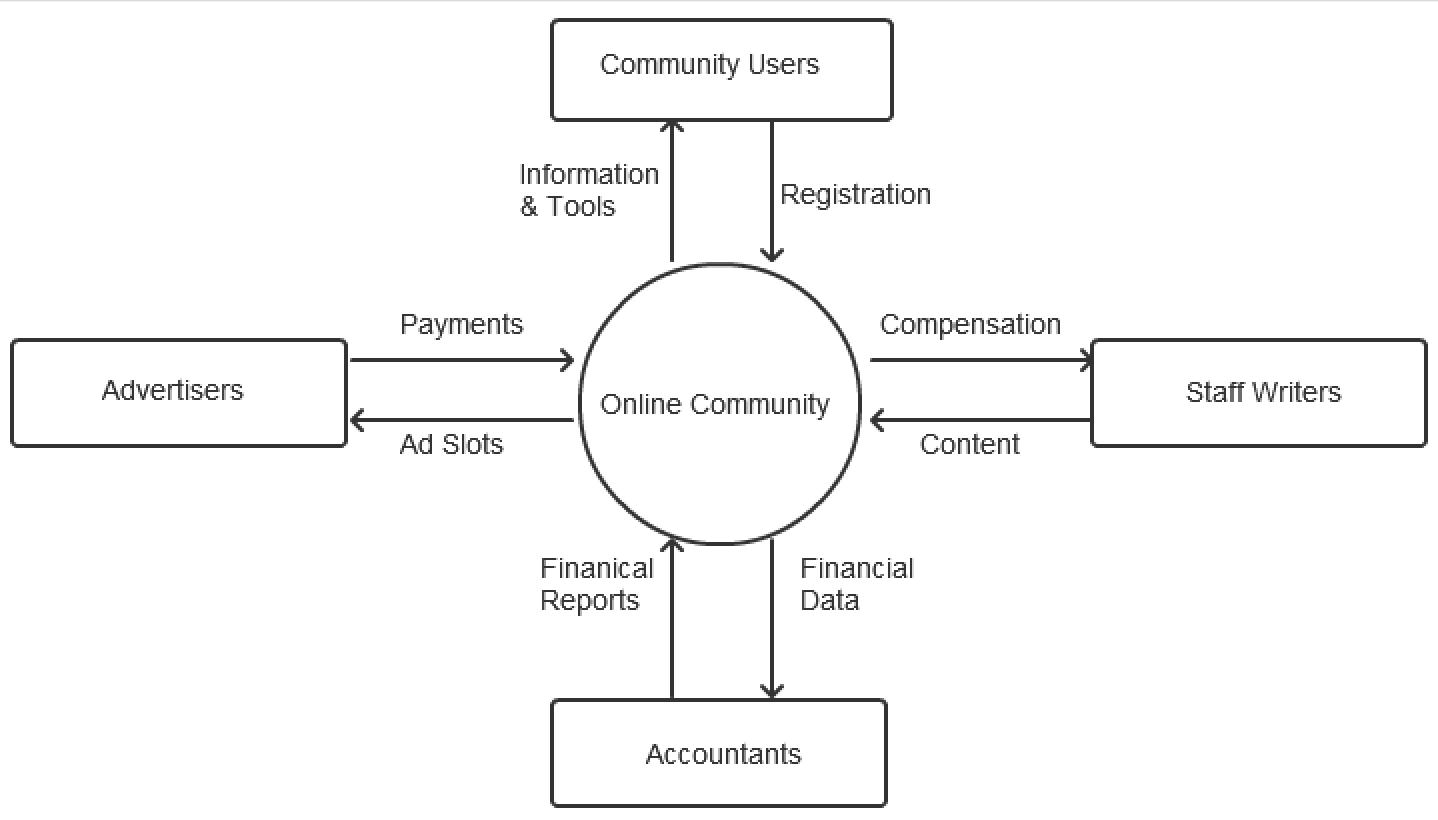
\includegraphics[width=0.9\textwidth]{Figures/Context Diagram.png}
\caption{Sample Context Diagram of Proposed System}
\label{fig:usecase}
\end{figure}

\textbf{Guidelines:}
\begin{itemize}
    \item Show system boundary.
    \item Include users, admin, third-party APIs, databases, ML engines, payment gateways, etc.
    \item Keep diagram simple and high-level.
\end{itemize}

%%%%%%%%%%%%%%%%%%%%%%%%%%%%%%%%%%%%%%%%%%%%%%%%%%%%%%
\section{Architectural Design}

This section describes the high-level architecture of the system.

\begin{figure}[h]
\centering
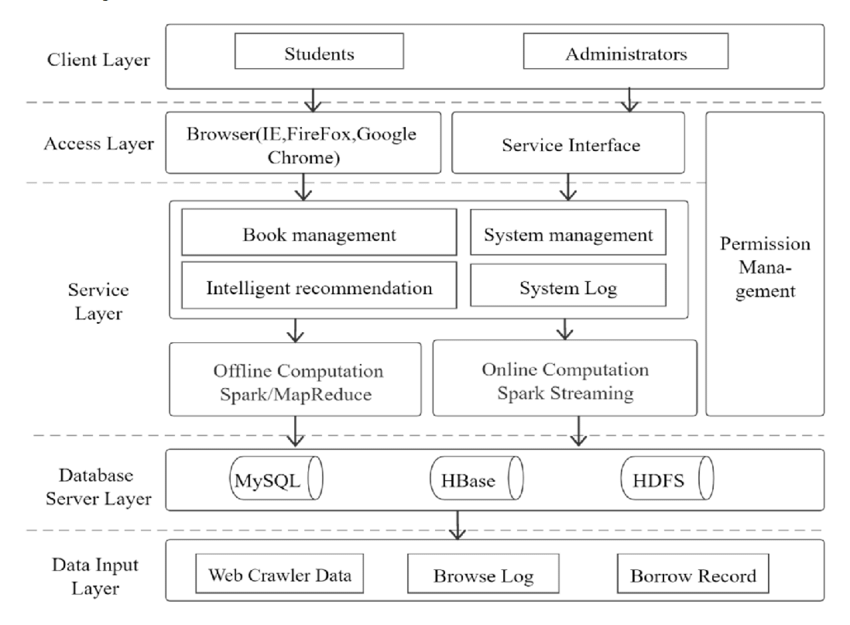
\includegraphics[width=0.9\textwidth]{Figures/Architecture Diagram.png}
\caption{Sample System Architecture Diagram of Proposed System}
\label{fig:usecase}
\end{figure}


\textbf{Guidelines:}
\begin{itemize}
    \item Divide system into layers (Presentation, Business Logic, Data Layer).
    \item For ML projects, include:
        \begin{itemize}
            \item Data Preprocessing Module
            \item Model Training Module
            \item Prediction Engine
            \item Evaluation Module
        \end{itemize}
    \item For Web/Mobile:
        \begin{itemize}
            \item Frontend
            \item Backend
            \item API Layer
            \item Database
        \end{itemize}
    \item Explain interaction between components.
\end{itemize}


%%%%%%%%%%%%%%%%%%%%%%%%%%%%%%%%%%%%%%%%%%%%%%%%%%%%%%
\section{Design Models}

This section presents detailed design models of the system. These models describe system behavior, structure, and interactions using UML diagrams. The models help developers understand system workflow before implementation.

%%%%%%%%%%%%%%%%%%%%%%%%%%%%%%%%%%%%%%%%%%%%%%%%%%%%%%
\subsection{Activity Diagrams}

Activity diagrams represent the workflow of different modules of the system. Each core module must have a separate activity diagram.

\begin{figure}[h]
\centering
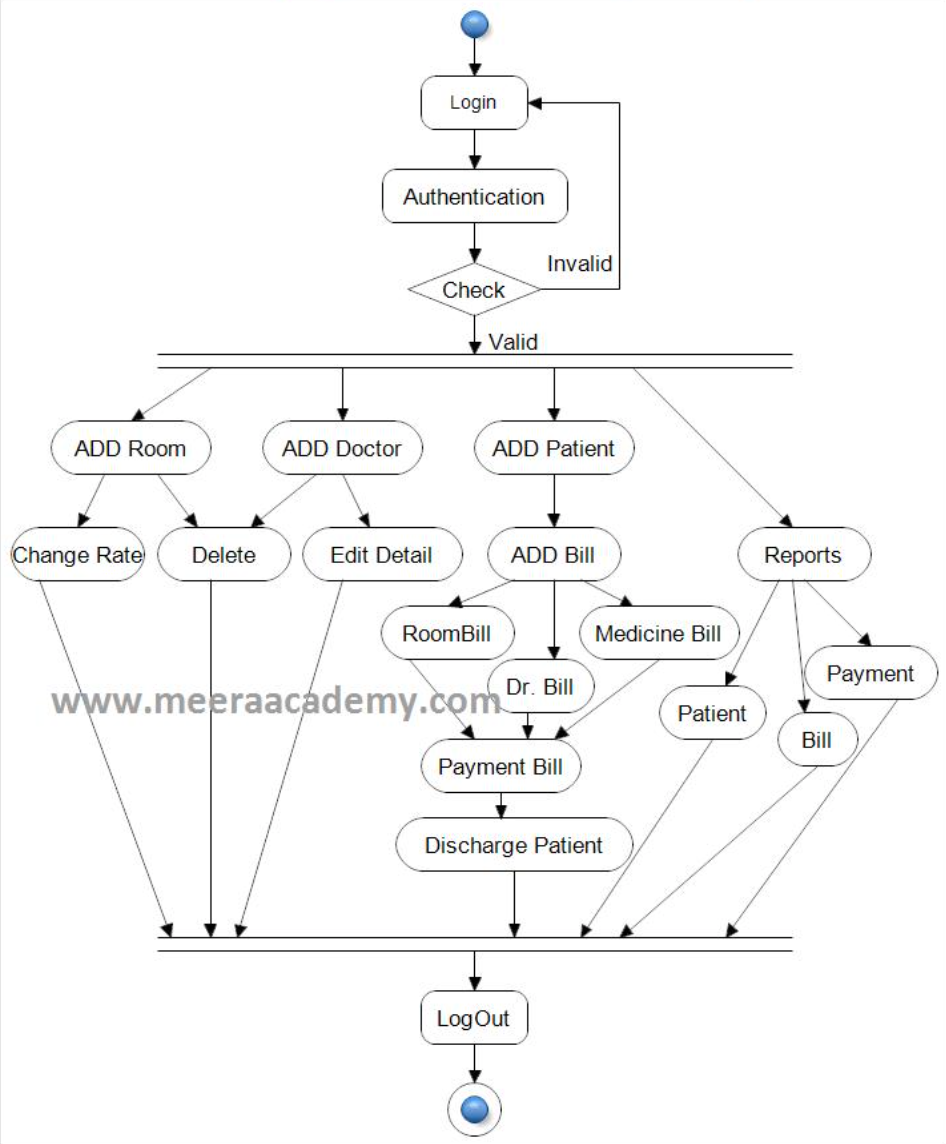
\includegraphics[width=0.67\textwidth]{Figures/Activity Diagram.png}
\caption{Sample Activity Diagram}
\label{fig:usecase}
\end{figure}

\textbf{Guidelines:}
\begin{itemize}
    \item Start with user interaction.
    \item Include decision nodes.
    \item Show validation checks.
    \item Include database/model interaction.
    \item Clearly indicate start and end states.
\end{itemize}

%%%%%%%%%%%%%%%%%%%%%%%%%%%%%%%%%%%%%%%%%%%%%%%%%%%%%%
\subsubsection{Module 1: User Management}

\textbf{Description:}
This diagram illustrates user registration, login, authentication, and profile management processes.

\textbf{Figure 4.X: Activity Diagram – User Module}
%%%%%%%%%%%%%%%%%%%%%%%%%%%%%%%%%%%%%%%%%%%%%%%%%%%%%%
\subsubsection{Module 2: Core Functional Module}

(Examples depending on domain)

For ML:
- Data Upload
- Model Training
- Prediction Generation

For Web/Mobile:
- Order Processing
- Search System
- Booking System

\textbf{Figure 4.X: Activity Diagram – Core Module}

%%%%%%%%%%%%%%%%%%%%%%%%%%%%%%%%%%%%%%%%%%%%%%%%%%%%%%
\subsubsection{Module 3: Admin Module}

\textbf{Figure 4.X: Activity Diagram – Admin Operations}

Include:
- Monitoring
- Reports
- Data Management
- User Control

%%%%%%%%%%%%%%%%%%%%%%%%%%%%%%%%%%%%%%%%%%%%%%%%%%%%%%
\subsection{Class Diagram}

The class diagram shows the static structure of the system.

\textbf{Figure 4.X: Class Diagram}

\textbf{Guidelines:}
\begin{itemize}
    \item Include classes, attributes, and methods.
    \item Show relationships (Association, Aggregation, Inheritance).
    \item For ML systems include:
        \begin{itemize}
            \item Dataset Class
            \item Model Class
            \item Evaluation Class
        \end{itemize}
    \item For Web/Mobile:
        \begin{itemize}
            \item User
            \item Admin
            \item Order/Transaction
            \item Service
        \end{itemize}
\end{itemize}

\begin{figure}[h]
\centering
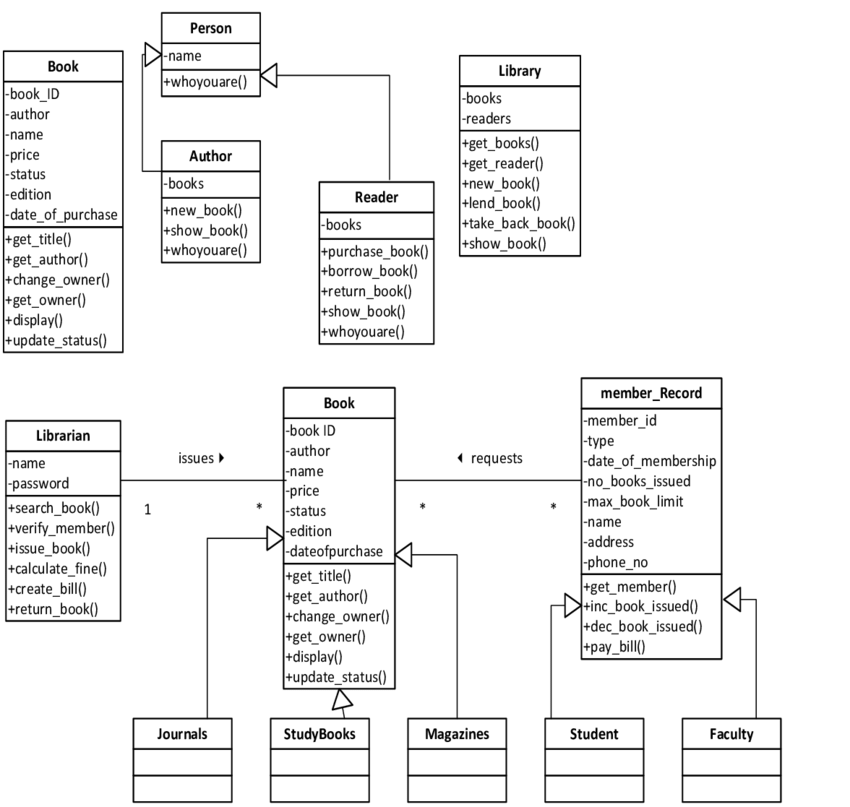
\includegraphics[width=0.88\textwidth]{Figures/Class Diagram.png}
\caption{Sample Class Diagram}
\label{fig:usecase}
\end{figure}

Include explanation after diagram describing:
\begin{itemize}
    \item Key classes
    \item Relationships
    \item Responsibilities
\end{itemize}

%%%%%%%%%%%%%%%%%%%%%%%%%%%%%%%%%%%%%%%%%%%%%%%%%%%%%%
\subsection{Sequence Diagrams}

Sequence diagrams show interaction between objects over time.

\textbf{Guidelines:}
\begin{itemize}
    \item Include actor on left.
    \item Show request-response flow.
    \item Include system components.
    \item Show database/API interaction.
\end{itemize}

%%%%%%%%%%%%%%%%%%%%%%%%%%%%%%%%%%%%%%%%%%%%%%%%%%%%%%
\subsubsection{Sequence Diagram – User Login}

\begin{figure}[h]
\centering
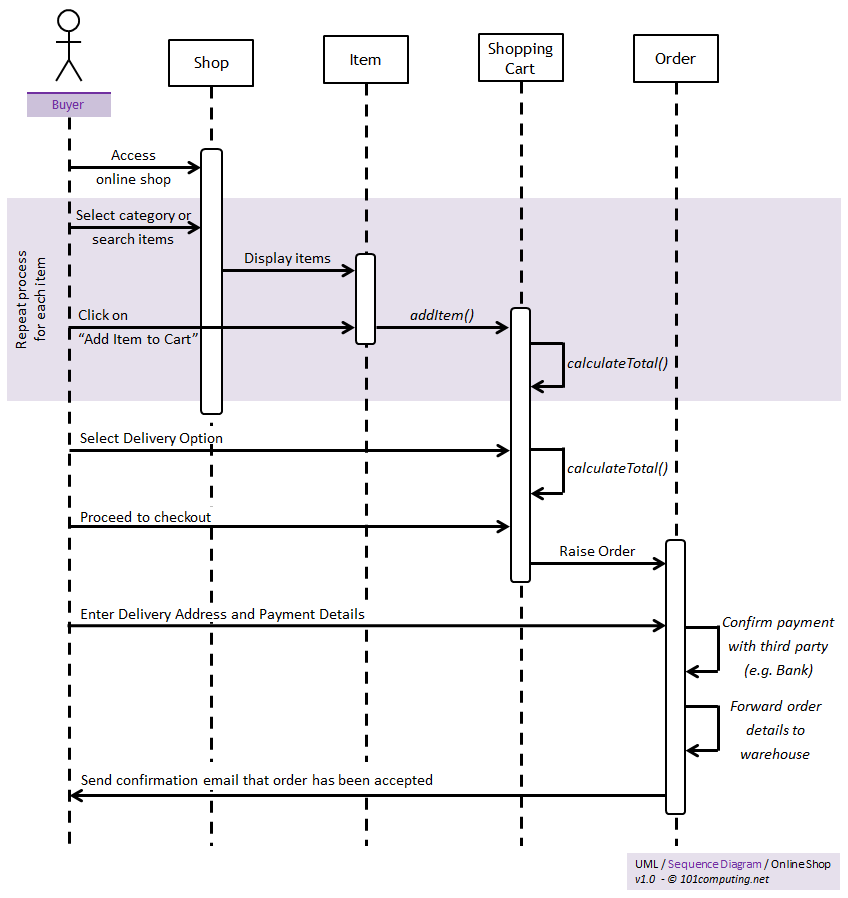
\includegraphics[width=0.8\textwidth]{Figures/Sequence Diagram 2.png}
\caption{Sample Sequence Diagram}
\label{fig:usecase}
\end{figure}

Describe:
- User sends credentials
- System validates
- Database checks
- Response returned
%%%%%%%%%%%%%%%%%%%%%%%%%%%%%%%%%%%%%%%%%%%%%%%%%%%%%%
\subsubsection{Sequence Diagram – Core Operation}

Examples:

For ML:
- Upload Dataset → Preprocess → Load Model → Predict → Display Result

For Web:
- Add to Cart → Checkout → Payment Gateway → Confirmation

\begin{figure}[h]
\centering
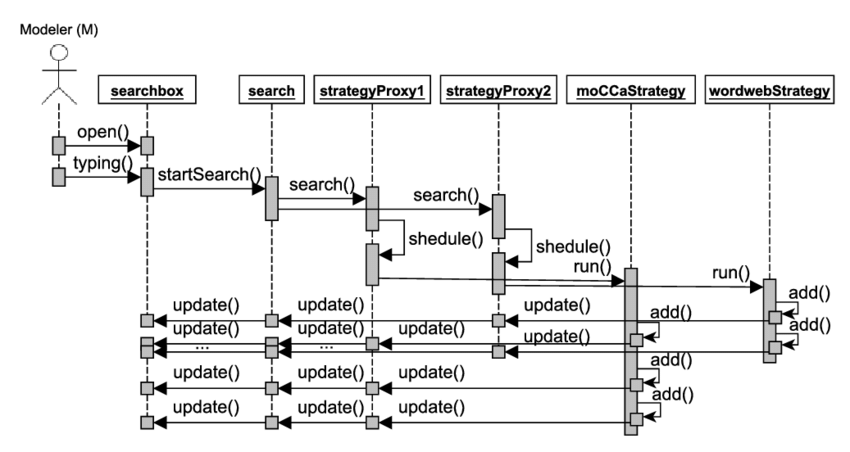
\includegraphics[width=0.8\textwidth]{Figures/Sequence Diagram.png}
\caption{Sample Sequence Diagram - 2}
\label{fig:usecase}
\end{figure}
%%%%%%%%%%%%%%%%%%%%%%%%%%%%%%%%%%%%%%%%%%%%%%%%%%%%%%
\subsection{State Transition Diagrams}

\begin{figure}[h]
\centering
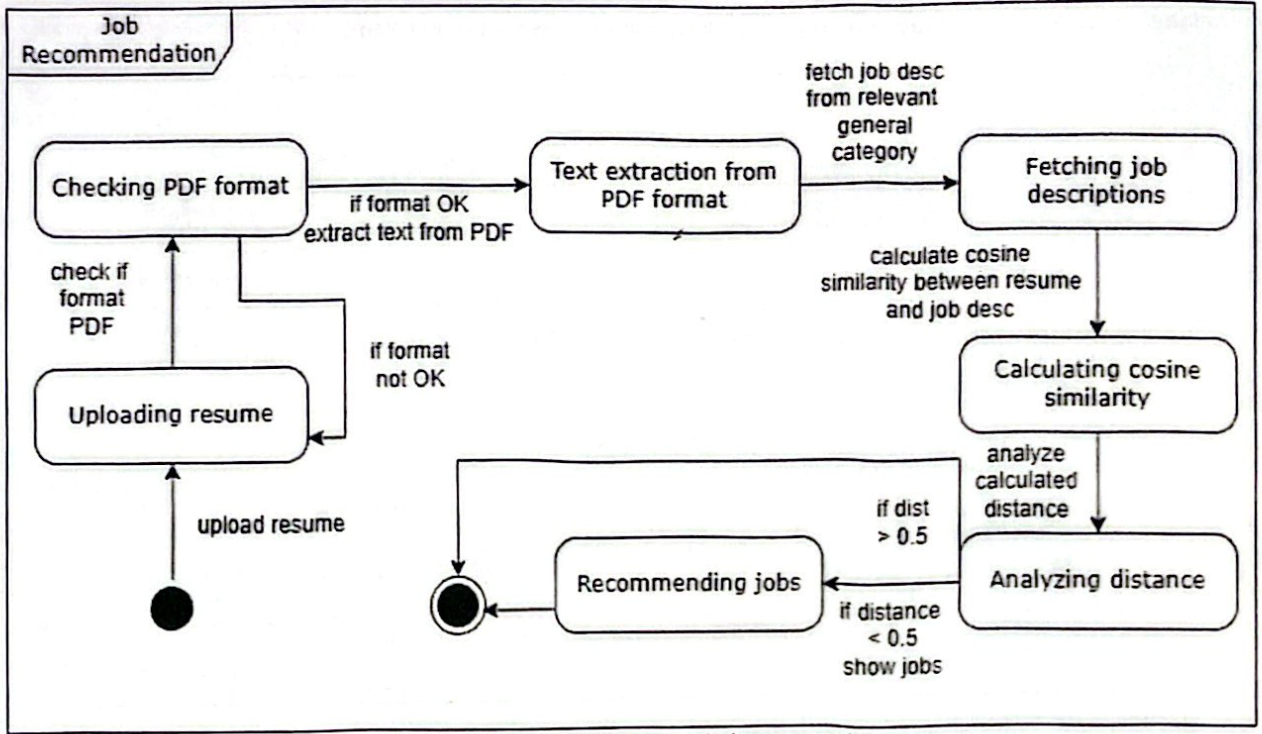
\includegraphics[width=0.77\textwidth]{Figures/State Transition.png}
\caption{Sample State Transition Diagram}
\label{fig:usecase}
\end{figure}

State diagrams show how system or object changes states over time.

\textbf{Examples:}
\begin{itemize}
    \item User Account States (Registered → Active → Suspended → Deleted)
    \item Order States (Created → Paid → Shipped → Delivered)
    \item ML Model States (Initialized → Training → Trained → Deployed)
\end{itemize}

\textbf{Guidelines:}
\begin{itemize}
    \item Clearly define states.
    \item Show triggering events.
    \item Include transitions with conditions.
\end{itemize}
%%%%%%%%%%%%%%%%%%%%%%%%%%%%%%%%%%%%%%%%%%%%%%%%%%%%%%
\section{Data Flow Diagrams}

Data Flow Diagrams (DFD) describe how data moves within the system. 
Different levels of DFD provide increasing detail.

\subsection{Level 1 Data Flow Diagram}

\begin{figure}[h]
\centering
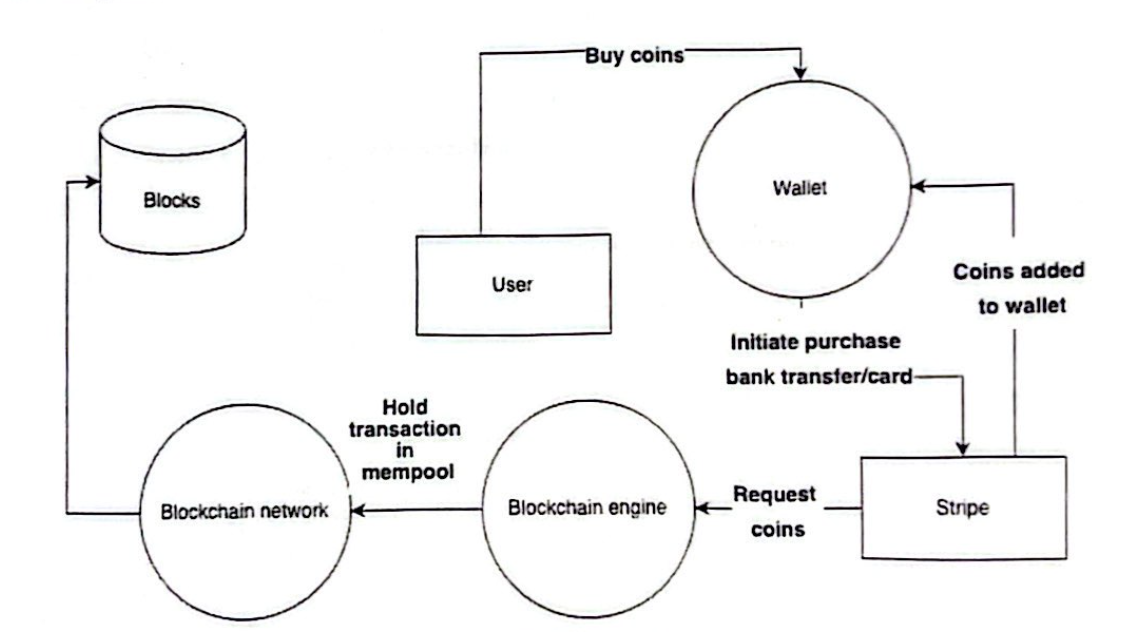
\includegraphics[width=0.9\textwidth]{Figures/DFD Sample.png}
\caption{Sample Level 1 DFD}
\label{fig:usecase}
\end{figure}  

\textbf{Description:}
Level 1 DFD decomposes the main system into major sub-processes.

\textbf{Include:}
\begin{itemize}
    \item Authentication Module
    \item Core Functional Module
    \item Data Processing Module
    \item Admin Module
    \item Database/Data Store
\end{itemize}

\textbf{Guidelines:}
\begin{itemize}
    \item Show internal processes.
    \item Show data stores.
    \item Maintain data flow consistency with Level 0.
\end{itemize}

%%%%%%%%%%%%%%%%%%%%%%%%%%%%%%%%%%%%%%%%%%%%%%%%%%%%%%
\subsection{Level 2 Data Flow Diagram}

\textbf{Description:}
Level 2 DFD further decomposes one complex module from Level 1.  

\begin{figure}[h]
\centering
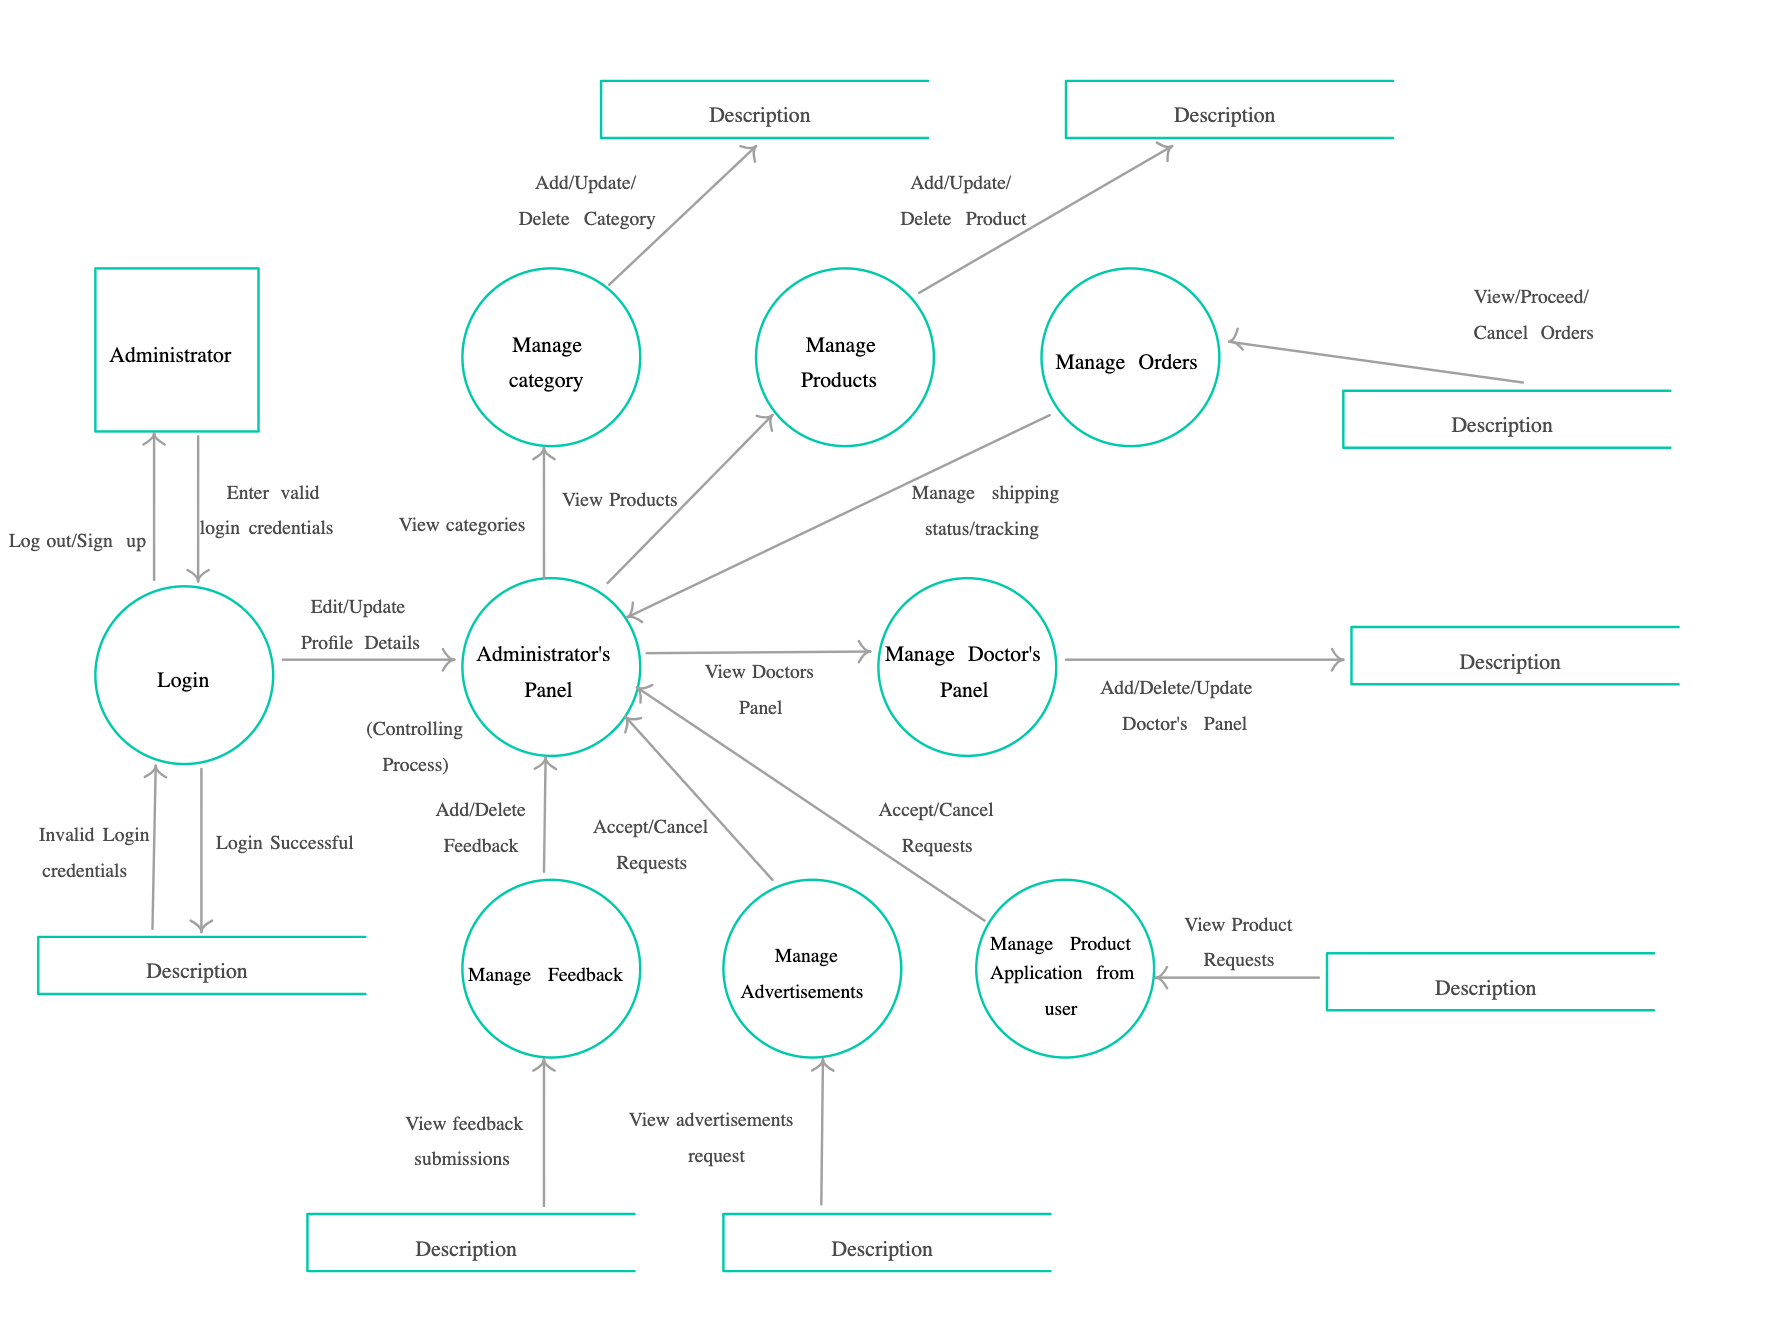
\includegraphics[width=0.9\textwidth]{Figures/DFD Sample 2.png}
\caption{Sample Level 2 DFD}
\label{fig:usecase}
\end{figure} 

\textbf{Examples (Domain-based):}

For Machine Learning:
\begin{itemize}
    \item Data Upload
    \item Data Preprocessing
    \item Model Training
    \item Prediction Generation
\end{itemize}

For Web/Mobile:
\begin{itemize}
    \item Cart Processing
    \item Payment Handling
    \item Booking Workflow
\end{itemize}

For Blockchain:
\begin{itemize}
    \item Transaction Validation
    \item Consensus Mechanism
    \item Block Creation
\end{itemize}

%%%%%%%%%%%%%%%%%%%%%%%%%%%%%%%%%%%%%%%%%%%%%%%%%%%%%%
\section{Data Design}

This section describes how data is structured, stored, and managed.

\textbf{Guidelines:}
\begin{itemize}
    \item Define database type (SQL / NoSQL).
    \item Explain schema structure.
    \item Describe indexing strategy.
    \item Mention security mechanisms.
    \item Discuss scalability considerations.
\end{itemize}

%%%%%%%%%%%%%%%%%%%%%%%%%%%%%%%%%%%%%%%%%%%%%%%%%%%%%%
\subsection{Entity Relationship Diagram (ERD)}

\begin{figure}[h]
\centering
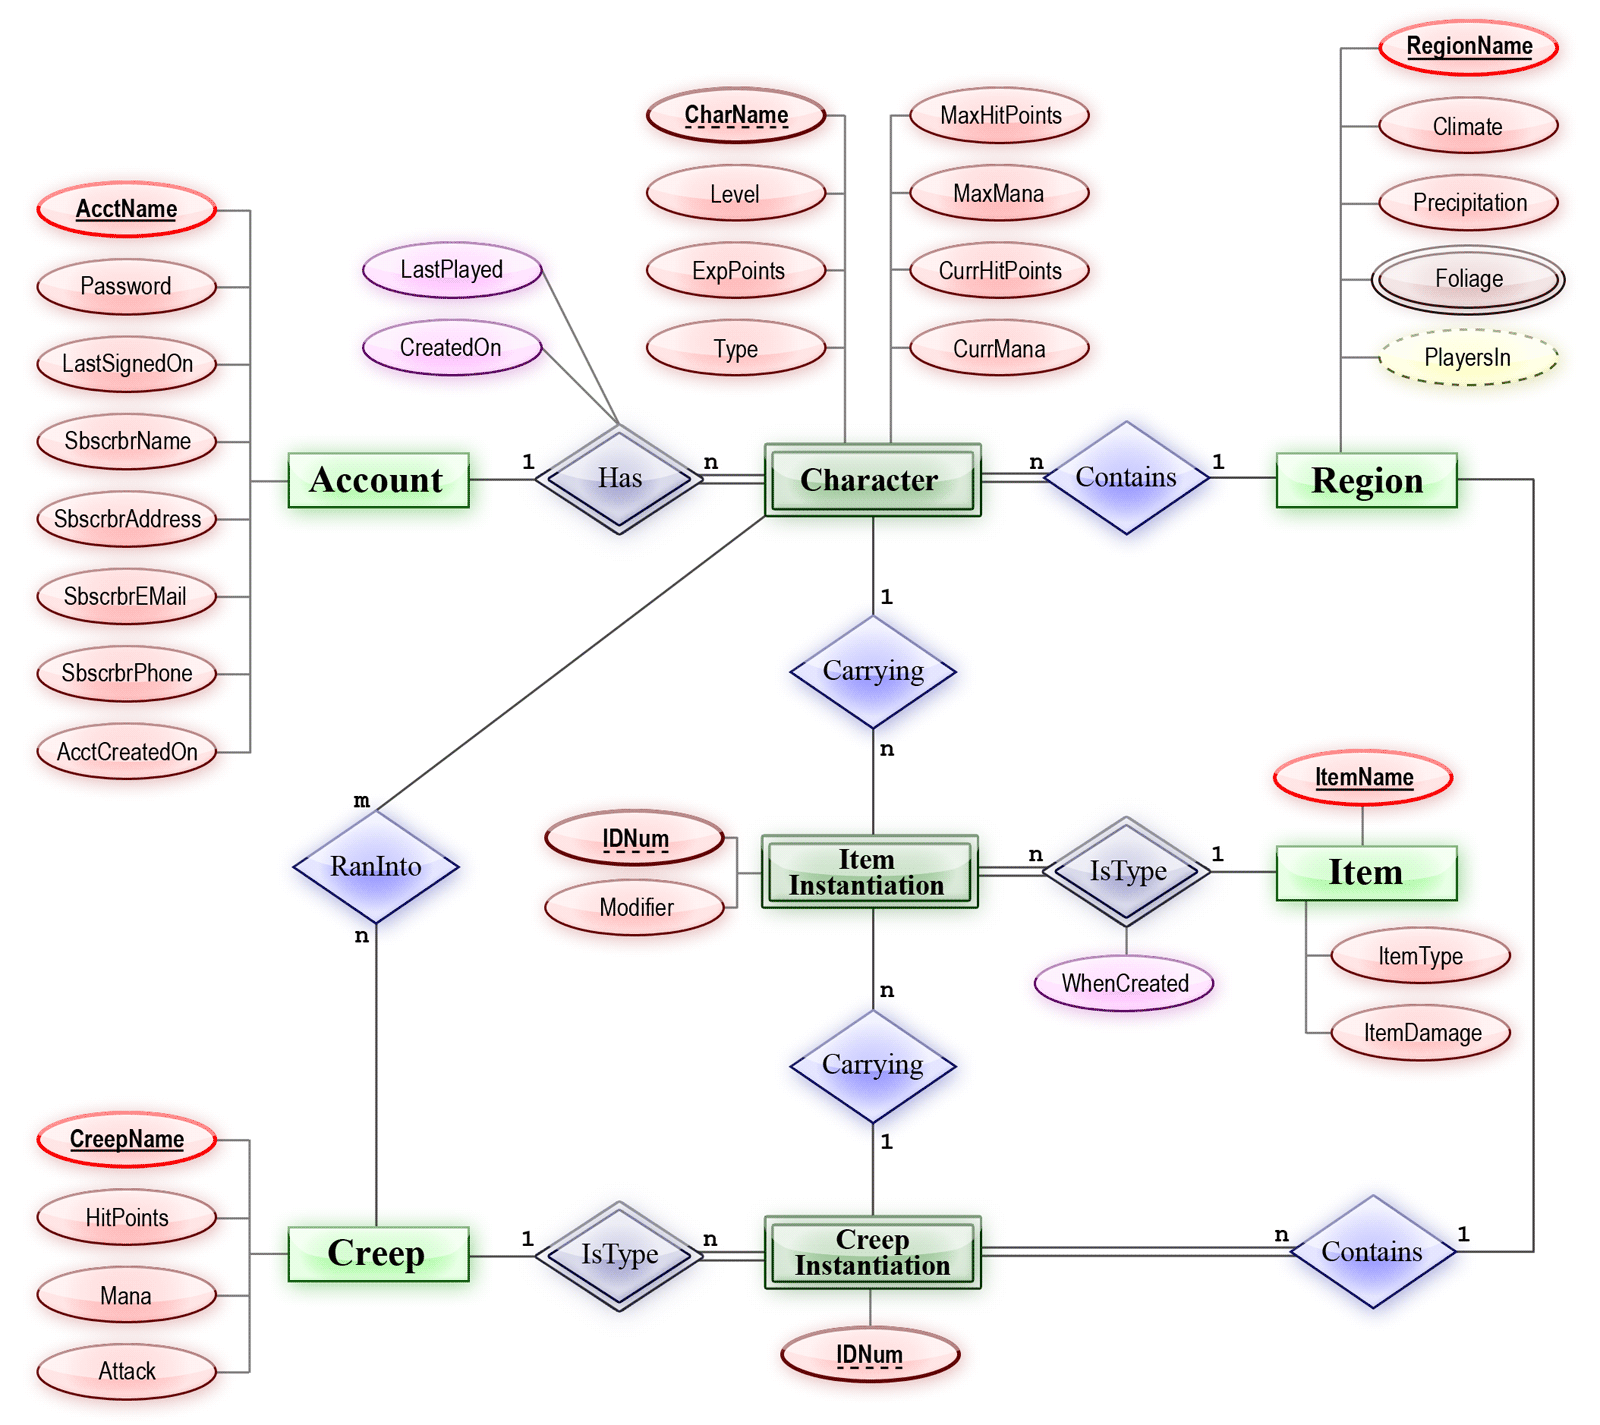
\includegraphics[width=0.9\textwidth]{Figures/ER Diagram.png}
\caption{Sample Entity Relation Diagram}
\label{fig:usecase}
\end{figure} 

The Entity Relationship Diagram (ERD) represents the logical database structure of the system. 

\textbf{Guidelines:}
\begin{itemize}
    \item Clearly identify all entities (tables/collections).
    \item Highlight Primary Keys (PK).
    \item Highlight Foreign Keys (FK).
    \item Show relationship cardinality (1:1, 1:N, M:N).
    \item Maintain consistency with database tables defined earlier.
\end{itemize}

\textbf{Include in ERD:}
\begin{itemize}
    \item User Entity
    \item Core Functional Entities (domain-based)
    \item Transaction/Log Entity
    \item Administrative Entity (if applicable)
\end{itemize}



%%%%%%%%%%%%%%%%%%%%%%%%%%%%%%%%%%%%%%%%%%%%%%%%%%%%%%
\subsection{Database Architecture}

Explain:
\begin{itemize}
    \item Client-Server Architecture
    \item Cloud Storage (if applicable)
    \item Distributed Storage (for Blockchain/ML)
\end{itemize}

%%%%%%%%%%%%%%%%%%%%%%%%%%%%%%%%%%%%%%%%%%%%%%%%%%%%%%
\section{Database Schema Diagram}

\begin{figure}[h]
\centering
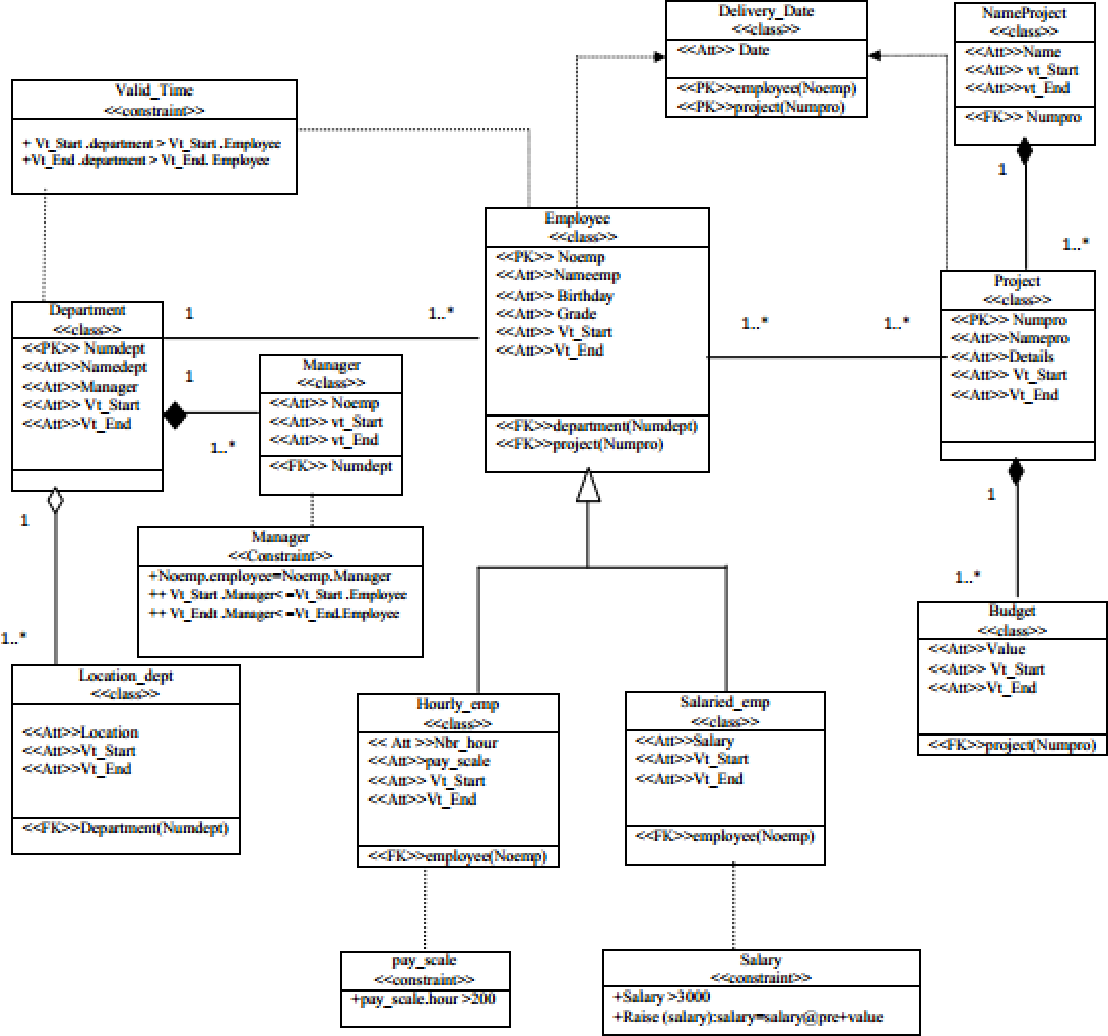
\includegraphics[width=0.9\textwidth]{Figures/Database Diagram.png}
\caption{Sample Database Diagram}
\label{fig:usecase}
\end{figure} 

The Database Schema Diagram represents the physical database implementation structure.

\textbf{Guidelines:}
\begin{itemize}
    \item Show actual table structure.
    \item Include column names and data types.
    \item Show PK and FK relationships.
    \item Reflect normalization level (1NF, 2NF, 3NF if applicable).
\end{itemize}

\textbf{Explanation (50–80 words in final report):}
Explain how the schema supports:
\begin{itemize}
    \item Data integrity
    \item Efficient querying
    \item Scalability
    \item Security
\end{itemize}


%%%%%%%%%%%%%%%%%%%%%%%%%%%%%%%%%%%%%%%%%%%%%%%%%%%%%%
\subsection{Data Dictionary}

Data Dictionary defines structure of all data elements.

\textbf{Guidelines:}
\begin{itemize}
    \item Include field name
    \item Data type
    \item Size
    \item Description
    \item Constraints
\end{itemize}

%%%%%%%%%%%%%%%%%%%%%%%%%%%%%%%%%%%%%%%%%%%%%%%%%%%%%%
\begin{table}[h]
\centering
\caption{Sample Data Dictionary – User Table}
\begin{tabularx}{\textwidth}{|p{3cm}|p{2cm}|p{2cm}|X|}
\hline
\textbf{Field Name} & \textbf{Type} & \textbf{Size} & \textbf{Description} \\
\hline
user\_id & INT & 11 & Unique identifier for each user \\
\hline
username & VARCHAR & 100 & Name chosen by user \\
\hline
email & VARCHAR & 150 & Registered email address \\
\hline
password & VARCHAR & 255 & Encrypted password \\
\hline
role & VARCHAR & 50 & User type (Admin/User) \\
\hline
\end{tabularx}
\end{table}

%%%%%%%%%%%%%%%%%%%%%%%%%%%%%%%%%%%%%%%%%%%%%%%%%%%%%%
%===========================================================
\section{Database Tables / Collections}
%===========================================================

This section describes the logical database design of the system. It presents the major relational tables (for SQL-based systems) or collections (for NoSQL-based systems). The database structure is designed to ensure data consistency, integrity, security, and scalability.

Each table or collection includes primary keys, relationships, and major attributes relevant to system functionality.



%%%%%%%%%%%%%%%%%%%%%%%%%%%%%%%%%%%%%%%%%%%%%%%%%%%%%%
\subsection{User Collection / Table}
%%%%%%%%%%%%%%%%%%%%%%%%%%%%%%%%%%%%%%%%%%%%%%%%%%%%%%

The User table stores authentication credentials and user profile information. It supports role-based access control and secure authentication.

\textbf{Description:}
\begin{itemize}
    \item Primary Key: \texttt{user\_id}
    \item Relationships: Linked to transactions, predictions, or system logs.
    \item Authentication Attributes: Email, password hash, role, account status.
\end{itemize}

\begin{table}[h]
\centering
\caption{User Table Structure}

\begin{tabularx}{\textwidth}{|p{3cm}|p{3cm}|p{3cm}|X|}
\hline
\textbf{Field Name} & \textbf{Data Type} & \textbf{Constraint} & \textbf{Description} \\
\hline
user\_id & INT / UUID & Primary Key & Unique identifier for each user \\
\hline
full\_name & VARCHAR(100) & Not Null & Stores user’s full name \\
\hline
email & VARCHAR(150) & Unique, Not Null & User login email address \\
\hline
password\_hash & VARCHAR(255) & Not Null & Encrypted password using hashing algorithm \\
\hline
role & VARCHAR(50) & Not Null & Defines user access level (Admin, User, etc.) \\
\hline
created\_at & TIMESTAMP & Default Current & Account creation timestamp \\
\hline
status & BOOLEAN & Default True & Indicates whether account is active \\
\hline
\end{tabularx}

\end{table}



%%%%%%%%%%%%%%%%%%%%%%%%%%%%%%%%%%%%%%%%%%%%%%%%%%%%%%
\subsection{Core Data Collection}
%%%%%%%%%%%%%%%%%%%%%%%%%%%%%%%%%%%%%%%%%%%%%%%%%%%%%%

This subsection describes domain-specific core data tables or collections. These structures store primary operational data processed by the system.

\textbf{Domain-Specific Examples:}

\textbf{For Machine Learning Systems:}
\begin{itemize}
    \item Dataset Collection – Stores training and testing datasets.
    \item Model Metadata Collection – Stores model version, hyperparameters, and evaluation metrics.
    \item Prediction Results Collection – Stores inference results and timestamps.
\end{itemize}

\textbf{For Web-Based Systems:}
\begin{itemize}
    \item Orders Table – Stores customer purchase records.
    \item Products Table – Stores product details and pricing.
    \item Transactions Table – Stores payment and transaction history.
\end{itemize}

\textbf{For Mobile Applications:}
\begin{itemize}
    \item Device Info Table – Stores device metadata.
    \item Session Table – Tracks active user sessions.
\end{itemize}

\textbf{For Blockchain-Based Systems:}
\begin{itemize}
    \item Transaction Collection – Stores blockchain transaction records.
    \item Wallet Collection – Stores wallet identifiers and balances.
    \item Block Metadata Collection – Stores block hash, timestamp, and validation status.
\end{itemize}



%%%%%%%%%%%%%%%%%%%%%%%%%%%%%%%%%%%%%%%%%%%%%%%%%%%%%%
\subsection{Relationships Between Tables}
%%%%%%%%%%%%%%%%%%%%%%%%%%%%%%%%%%%%%%%%%%%%%%%%%%%%%%

Database relationships define how data entities are connected within the system.

\begin{itemize}
    \item \textbf{One-to-One (1:1):} Each user may have one profile detail record.
    \item \textbf{One-to-Many (1:N):} One user may generate multiple transactions or predictions.
    \item \textbf{Many-to-Many (M:N):} Users may interact with multiple products, and products may belong to multiple categories (resolved using junction tables).
\end{itemize}

An Entity-Relationship (ER) Diagram should be included to visually represent these relationships.



%%%%%%%%%%%%%%%%%%%%%%%%%%%%%%%%%%%%%%%%%%%%%%%%%%%%%%
\subsection{Security and Data Integrity}
%%%%%%%%%%%%%%%%%%%%%%%%%%%%%%%%%%%%%%%%%%%%%%%%%%%%%%

To ensure confidentiality and integrity of stored data, the following measures are implemented:

\begin{itemize}
    \item Password Encryption using secure hashing algorithms (e.g., bcrypt, SHA-256 with salt).
    \item Role-Based Access Control (RBAC) to restrict unauthorized access.
    \item Input validation and constraint enforcement at database level.
    \item Secure communication using HTTPS.
    \item Regular database backup and disaster recovery strategy.
\end{itemize}



%%%%%%%%%%%%%%%%%%%%%%%%%%%%%%%%%%%%%%%%%%%%%%%%%%%%%%
\subsection{Scalability Considerations}
%%%%%%%%%%%%%%%%%%%%%%%%%%%%%%%%%%%%%%%%%%%%%%%%%%%%%%

The database design incorporates scalability mechanisms to support future growth.

\begin{itemize}
    \item Horizontal Scaling using distributed database systems (if required).
    \item Indexing on frequently queried attributes to improve performance.
    \item Caching strategies for frequently accessed data.
    \item Load balancing across database instances.
    \item Partitioning or sharding for large-scale data environments.
\end{itemize}


%%%%%%%%%%%%%%%%%%%%%%%%%%%%%%%%%%%%%%%%%%%%%%%%%%%%%%
\section{Chapter Summary}
%%%%%%%%%%%%%%%%%%%%%%%%%%%%%%%%%%%%%%%%%%%%%%%%%%%%%%

This chapter presented the comprehensive software design of the proposed system. 
It translated the functional and non-functional requirements identified earlier 
into structured architectural, behavioral, and data models.

The design methodology and selected software process model were justified to 
ensure systematic development and maintainability. A high-level system overview 
was provided through the context diagram and architectural representation, 
clearly illustrating component interactions and subsystem boundaries.

Detailed UML models including activity diagrams, class diagrams, sequence diagrams, 
and state transition diagrams were developed to describe system behavior and structure. 
Additionally, data flow diagrams were constructed to represent internal data movement 
across different system layers.

The chapter further elaborated the database design through Entity Relationship Diagrams, 
database schema diagrams, and data dictionaries to ensure data integrity, scalability, 
and security. Relationships between entities and normalization considerations were 
also addressed.

Overall, this chapter establishes a clear technical blueprint that guides the 
implementation phase discussed in the next chapter.
